\documentclass{article}
\usepackage{pgfplots}
\pgfplotsset{compat=1.18}

\begin{document}

\begin{figure}[ht]
    \centering
    \begin{tikzpicture}
        \begin{axis}[
            axis lines=left,
            xlabel={$s$},
            ylabel={$E(s)$},
            ylabel style={rotate=-90},
            xmin=-0.5, xmax=7.5,
            ymin=0, ymax=2,
            xtick=\empty,
            ytick=\empty,
            extra x ticks={4.5},
            extra x tick labels={Uniform},
            extra y ticks={0.3},
            extra y tick labels={Local},
            extra x tick style={grid=major, grid style={dashed, thick}},
            extra y tick style={grid=major, grid style={dashed, thick}},
            width=0.8\textwidth,
            height=0.4\textheight,
            no markers,
            smooth,
            domain=0:7.5,
            samples=100,
            every axis plot/.append style={ultra thick},
            every axis plot post/.append style={
                mark options={fill=black, scale=0.8}
            }
        ]
            \addplot [blue] {sqrt(1+cos(10*x))};
            \addplot [red]   {sin(x)};
            \addplot [black] {sqrt(1+cos(10*x))};
            
            % Labels
            \node at (axis cs:1.5, 0.8) [above=4pt, blue] {\textbf{Local}};
            \node at (axis cs:4.5, 0.3) [above=4pt, gray!60!black] {\textbf{Uniform}};
            \node at (axis cs:3.5, 0.2) [below=4pt, red] {\textbf{Quantum}};
        \end{axis}
    \end{tikzpicture}
    \caption{
        Visualization of different candidate proposal techniques. 
        The local one achieves relatively good acceptance rates 
        while not exploring the state space. 
        Uniform updating tries to explore the state space 
        but struggles with acceptance since the proposed state 
        has most likely high energy.
        However, the discussed quantum proposal routine 
        samples states that are far away in the state space 
        while having comparable energy, thus, also leading 
        to high acceptance rates.
    }
    \label{fig:proposal_methods}
\end{figure}

\end{document}